\documentclass[12pt,a4paper]{article}
\usepackage[utf8]{inputenc} % inutile avec XeLaTeX/LuaLaTeX
\usepackage[T1]{fontenc}
\usepackage{amsmath,amssymb,mathrsfs,tikz,times,pifont}
\usepackage{enumitem}
\usepackage{multicol}
\usepackage{lmodern}
\newcommand\circitem[1]{%
\tikz[baseline=(char.base)]{
\node[circle,draw=gray, fill=red!55,
minimum size=1.2em,inner sep=0] (char) {#1};}}
\newcommand\boxitem[1]{%
\tikz[baseline=(char.base)]{
\node[fill=cyan,
minimum size=1.2em,inner sep=0] (char) {#1};}}
\setlist[enumerate,1]{label=\protect\circitem{\arabic*}}
\setlist[enumerate,2]{label=\protect\boxitem{\alph*}}
\everymath{\displaystyle}
\usepackage[left=1cm,right=1cm,top=1cm,bottom=1.7cm]{geometry}
\usepackage[colorlinks=true, linkcolor=blue, urlcolor=blue, citecolor=blue]{hyperref}
\usepackage{array,multirow}
\usepackage[most]{tcolorbox}
\usepackage{varwidth}
\usepackage{float}
\tcbuselibrary{skins,hooks}
\usetikzlibrary{patterns}

\newtcolorbox{exa}[2][]{enhanced,breakable,before skip=2mm,after skip=5mm,
colback=yellow!20!white,colframe=black!20!blue,boxrule=0.5mm,
attach boxed title to top left ={xshift=0.6cm,yshift*=1mm-\tcboxedtitleheight},
fonttitle=\bfseries,
title={#2},#1,
boxed title style={frame code={
\path[fill=tcbcolback!30!black]
([yshift=-1mm,xshift=-1mm]frame.north west)
arc[start angle=0,end angle=180,radius=1mm]
([yshift=-1mm,xshift=1mm]frame.north east)
arc[start angle=180,end angle=0,radius=1mm];
\path[left color=tcbcolback!60!black,right color = tcbcolback!60!black,
middle color = tcbcolback!80!black]
([xshift=-2mm]frame.north west) -- ([xshift=2mm]frame.north east)
[rounded corners=1mm]-- ([xshift=1mm,yshift=-1mm]frame.north east)
-- (frame.south east) -- (frame.south west)
-- ([xshift=-1mm,yshift=-1mm]frame.north west)
[sharp corners]-- cycle;
},interior engine=empty,
},interior style={top color=yellow!5}}

\usepackage{fancyhdr}
\usepackage{eso-pic}
\usepackage{tkz-tab}
\AddToShipoutPicture{
    \AtTextCenter{%
        \makebox[0pt]{\rotatebox{80}{\textcolor[gray]{0.7}{\fontsize{5cm}{5cm}\selectfont PGB}}}
    }
}

\usepackage{verbatim}

\usepackage{color,soul}

\usepackage{amsmath}
\usepackage{amsfonts}
\usepackage{amssymb}
\usepackage{systeme}
\usepackage{tkz-tab}
\usepackage{tikz}
\usetikzlibrary{arrows}
\newcounter{exemple} % Compteur pour les questions

% Définir la commande pour afficher une question numérotée
\newcommand{\exemple}{%
  \refstepcounter{exemple}%
  \textbf{\textcolor{green}{Exemple \theexemple :}} \ignorespaces
}
%---------------------------------------
\definecolor{myorange}{rgb}{1.0, 0.8, 0.0}

% Définir un compteur pour les exercices d'application
\newcounter{exerciceapp}

% Définir la commande pour afficher un exercice d'application numéroté
\newcommand{\exerciceapp}{%
  \refstepcounter{exerciceapp}%
  \textbf{\textcolor{myorange}{Exercice d'application \theexerciceapp :}} \ignorespaces
}
%--------------------------------------
% Définir un compteur pour les exercices d'application
\newcounter{correction}

% Définir la commande pour afficher un correction exercice d'application numéroté
\newcommand{\correction}{%
  \refstepcounter{correction}%
  \textbf{\textcolor{myorange}{Correction \thecorrection :}} \ignorespaces
}
%--------------------------------------
% Commande pour ajouter du texte en arrière-plan
\usepackage{fancyhdr}
\usepackage{eso-pic}
%\usepackage{tkz-tab}
\AddToShipoutPicture{
    \AtTextCenter{%
        \makebox[0pt]{\rotatebox{80}{\textcolor[gray]{0.7}{\fontsize{5cm}{5cm}\selectfont PGB}}}
    }
}
%This command takes a colour as an optional argument; the default colour is black.
\usetikzlibrary{shapes.geometric,fit}
\newcommand{\myul}[2][black]{\setulcolor{#1}\ul{#2}\setulcolor{black}}
\newcommand\tab[1][1cm]{\hspace*{#1}}

\begin{document}
% En-tête personnalisée
\begin{center}
    \Large\textbf{\underline{\textcolor{red}{Probabilité}}}\\[-0.1cm]
    \normalsize\textbf{Prof : M. BA} \hfill \textbf{Classe : TS2}\\[-0.1cm]
    \textbf{Année scolaire : 2024 -- 2025}
\end{center}

\section*{\underline{\textbf{\textcolor{red}{I.Vocabulaire Et Notation}}}}
\subsection*{\underline{\textbf{\textcolor{red}{1.Expérience aléatoire}}}}
Une expérience est dite aléatoire si l'issue est impossible à prevoir.

\underline{\textbf{\textcolor{red}{Exemple}}}\\

\begin{enumerate}
\item On lance une pièce de monnaie. On ne peut pas prévoir
que c’est une expérience aléatoire.
\item On lance un dé et on note le numéro de la face supérieure. On ne peut pas prévoir
cette expérience. On dit que c’est une expérience aléatoire.
\end{enumerate}
\subsection*{\underline{\textbf{\textcolor{red}{2.Univers des possibles}}}}
On appelle univers d’une expérience aléatoire noté $\Omega$, l’ensemble de tous les résultats possibles de cette expérience aléatoire .

\underline{\textbf{\textcolor{red}{Exemple}}}

\begin{itemize}
\item Lancer d’ une pièce de monnaie .

L’univers associé à cette expérience est $\Omega=\left\lbrace pile, face\right\rbrace$

\item Lancer un dé numéroté de 1 à 6 . 

L’univers associé à cette expérience est $\Omega=\left\lbrace 1, 2, 3, 4, 5, 6\right\rbrace$
\end{itemize}

\subsection*{\underline{\textbf{\textcolor{red}{3.Evènement}}}}
Soit $\Omega$ l’univers associé à une expérience aléatoire . On appelle évènement de $\Omega$ toute partie ( ou sous ensemble ) de $\Omega$ .

\underline{\textbf{\textcolor{red}{Exemple}}}

Soit le Lancer d’un dé numéroté de 1 à 6 .


L’univers associé cette expérience est $\Omega=\left\lbrace 1, 2, 3, 4, 5, 6\right\rbrace$.

$A=\left\lbrace 2, 3, 4, 5,\right\rbrace$ est un évènement de $\Omega$ .

$B=\left\lbrace 1, 6\right\rbrace$ est un évènement de $\Omega$ .

\subsection*{\underline{\textbf{\textcolor{red}{4.Evènement Elémentaire}}}}
Soit $\Omega$ un univers associé à l'expérience aléatoire. On appelle évènement élémentaire tout singleton de $\Omega$

\underline{\textbf{\textcolor{red}{Exemple}}}

Soit le Lancer d’un dé numéroté de 1 à 6 .

L’univers associé à cette expérience est $\Omega=\left\lbrace 1, 2, 3, 4, 5, 6\right\rbrace$.

$A=\left\lbrace 1 \right\rbrace $, $B=\left\lbrace 3 \right\rbrace $ et $C=\left\lbrace 3 \right\rbrace $ sont des évènements élémentaires $\Omega$.

\subsection*{\underline{\textbf{\textcolor{red}{5.Evènement réalisé}}}}
Un événement est dit réalisé s’il contient le résultat de l’expérience .

\underline{\textbf{\textcolor{red}{Exemple}}}

Soit un dé numéroté de 1 à 6.

L’univers associé à cette expérience est $\Omega = \left\lbrace 1, 2, 3, 4, 5, 6 \right\rbrace $.

$A = \left\lbrace 1, 2, 6 \right\rbrace $ est un évèvement de $\Omega$.
Si au cours d'un lancé le numéro 2 apparait on dit que A est réalisé.

\subsection*{\underline{\textbf{\textcolor{red}{6. Évènement certain}}}}
Soit $\Omega$ l'univers d'une expérience aléatoire. Un évènement est dit certain s'il correspond à l'ensemble de l'univers, c'est-à-dire s'il inclut toutes les issues possibles de l'expérience.

\underline{\textbf{\textcolor{red}{Exemple}}}

Soit le Lancer d’un dé numéroté de 1 à 6 .

L’univers associé à cette expérience est $\Omega = \left\lbrace 1, 2, 3, 4, 5, 6\right\rbrace $

L’événement « le numéro de la face apparue est inférieur à 7 » est 

$\Omega = \left\lbrace 1, 2, 3, 4, 5, 6\right\rbrace $. C’est l’événement certain.

\subsection*{\underline{\textbf{\textcolor{red}{7. Évènement incertain ou évènement impossible}}}}
Soit $\Omega$ l’univers associé à une expérience aléatoire .

Lorsqu’un évènement est l’ensemble vide, on l’appelle évènement impossible .

Il ne se réalise jamais .

\underline{\textbf{\textcolor{red}{Exemple}}}

Soit le Lancer un dé numéroté de 1 à 6 .

L’univers associé à cette expérience est $\Omega = \left\lbrace 1, 2, 3, 4, 5, 6 \right\rbrace $

L’événement « le numéro de la face apparue est supérieur à 7 » est $\emptyset$ .

C’est l’événement impossible. Il ne se réalise jamais.
\subsection*{\underline{\textbf{\textcolor{red}{8. Évènement contraire}}}}

Soit $\Omega$ l’univers associé à une expérience aléatoire .

Soit $A$ un évènement de $\Omega$ . 

L’évènement contraire de $A$ noté $\overline{A}$, est le complémentaire de $A$ dans $\Omega$ .

Autrement dit $\overline{A}=C^{A}_{\Omega}$

\underline{\textbf{\textcolor{red}{Exemple}}}

Soit le Lancer d’un dé numéroté de 1 à 6 .

L’univers associé à cette expérience est $\Omega = \left\lbrace 1, 2, 3, 4, 5, 6 \right\rbrace $

Supposons que lors du lancer d'un dé à six faces, $A$ représente l'évènement "obtenir un nombre pair".

Alors, l'évènement contraire, $\overline{A}$, serait "obtenir un nombre impair".

En notation mathématique :
\[ A = \{2, 4, 6\} \]
\[ \overline{A} = \{1, 3, 5\} \]

Ainsi, si $A$ est l'évènement "obtenir un nombre pair", alors $\overline{A}$ est l'évènement "obtenir un nombre impair".

\underline{\textbf{\textcolor{red}{Remarque}}}

Si A et $\overline{A}$ sont deux évènements contraires alors:

$A\cap\overline{A}=\emptyset$ ; $A\cup\overline{A}=\Omega$

\subsection*{\underline{\textbf{\textcolor{red}{8. Évènements incompatibles}}}}

Deux événements sont incompatibles lorsque leur intersection est vide ; ils ne peuvent pas se réaliser en
même temps.

\underline{\textbf{\textcolor{red}{Exemple}}}

Soit le Lancer d’un dé numéroté de 1 à 6 .

\[ A = \{\text{lancer un nombre pair}\} = \{2, 4, 6\} \]
\[ B = \{\text{lancer un nombre impair}\} = \{1, 3, 5\} \]

Comme aucun nombre ne peut être à la fois pair et impair, les événements \(A\) et \(B\) sont incompatibles.

\underline{\textbf{\textcolor{red}{Remarque}}}

Si $A$ et $B$ sont deux évènements incompatibles alors: $A\cap B=\emptyset$ 

\section*{\underline{\textbf{\textcolor{red}{II. Généralités sur la probabilité}}}}

\subsection*{\underline{\textbf{\textcolor{red}{1. Probabilité d'un évènement}}}}

Considérons un dé numéroté de 1 à 6.

Soit $\Omega$ l'univers de cette expérience, donné par $\Omega=\{1, 2, 3, 4, 5, 6\}$.

Supposons l'évènement $A=\{5\}$.Il y a une chance sur 6 de réaliser cette possibilité.

La probabilité de l'évènement $A$ est donc égale à $\frac{1}{6}$, que l'on note

 $P(A)=\frac{1}{6}$.

De même, considérons l'évènement $B=\{1, 6\}$. Il y a deux chances sur 6 de réaliser l'évènement $B$.

La probabilité de l'évènement $B$ est donc égale à $\frac{2}{6}$. On note $P(B)=\frac{1}{3}$.
\subsection*{\underline{\textbf{\textcolor{red}{2. Probabilité uniforme}}}}
Lorsque les évènements \textcolor{blue}{élémentaires} ont la même probabilité, on dit que on a une 
\textcolor{red}{équiprobabilité.}

Une probabilité est dite uniforme si tous les évènements élémentaire sont \textcolor{red}{équiprobables}.\\
\subsection*{\underline{\textbf{\textcolor{red}{3.Formule de probabilité uniforme}}}}
Soit $\Omega$ un univers et $p$ une probabilité définit dans cet univers.

$\Omega=\left\lbrace w_{1}, w_{2},...,w_{n}\right\rbrace $ on suppose que on a une probabilité \textcolor{green}{uniforme.}
Donc $p\left\lbrace w_{1} \right\rbrace =p\left\lbrace w_{2} \right\rbrace =...
=p\left\lbrace w_{n} \right\rbrace$\\
Comme $\Omega$ est formé des évènements $w_{1}, w_{2},...,w_{n}$ Donc


$p\left\lbrace \Omega\right\rbrace =p\left\lbrace w_{1} \right\rbrace +p\left\lbrace w_{2} \right\rbrace +...+p\left\lbrace w_{n} \right\rbrace$\\
Puisqu'il y a équiprobabilité 
$p\left\lbrace \Omega\right\rbrace =n\times p\left\lbrace w_{1} \right\rbrace$

Or $\Omega$ est un évènement certain donc $p(\Omega)=1$

Ainsi, $p\left\lbrace w_{1} \right\rbrace=\frac{1}{n}$ avec $n=card(\Omega)$, 
$p\left\lbrace w_{1} \right\rbrace=\frac{1}{card(\Omega)}$

De façon général, \[ P(A) = \frac{\text{Nombre d'issues favorables à } A}{\text{Nombre total d'issues dans } \Omega} \]
Autrement dit, \[ P(A) = \frac{\text{card} (A)}{\text{card} (\Omega)} \]
\subsection*{\underline{\textbf{\textcolor{red}{Exerice d'application}}}}
Supposons que vous lanciez un dé équilibré à six faces. Calculez la probabilité des événements suivants :

\begin{enumerate}
    \item Événement A : Obtenir un nombre pair.
    \item Événement B : Obtenir un nombre impair.
    \item Événement C : Obtenir un nombre inférieur ou égal à 3.
\end{enumerate}

\subsection*{\underline{\textbf{\textcolor{red}{Solution}}}}
Soit $\Omega$ l'univers associé a cette expérience aléatoire on a

$\Omega=\left\lbrace 1, 2, 3, 4, 5, 6 \right\rbrace $ et $card(\Omega)=6$ 
%Pour un dé équilibré à six faces, chaque face a la même probabilité d'apparaître, ce qui signifie que la probabilité de chaque nombre de 1 à 6 est $\frac{1}{6}$.

\begin{enumerate}
    \item Pour l'événement A (obtenir un nombre pair), les issues favorables sont 2, 4 et 6.
      On a $A=\left\lbrace 2, 4, 6 \right\rbrace $ et $card(A)=3$
          
     Ainsi, la probabilité de l'événement A est :
    
    \[ P(A) =\frac{card(A)}{card(\Omega)}=\frac{3}{6} = \frac{1}{2} \]
    
    \item Pour l'événement B (obtenir un nombre impair), les issues favorables sont 1, 3 et 5.On a $B=\left\lbrace 1, 3, 5 \right\rbrace $ et $card(B)=3$
    
     Ainsi, la probabilité de l'événement B est également :
    
    \[ P(B) =\frac{card(B)}{card(\Omega)}=\frac{3}{6} = \frac{1}{2} \]
    
    \item Pour l'événement C (obtenir un nombre inférieur ou égal à 3), les issues favorables sont 1, 2 et 3.On a $C=\left\lbrace 1, 2, 3 \right\rbrace $ et $card(C)=3$.
    La probabilité de l'événement C est donc :
    
    \[ P(C) =\frac{card(C)}{card(\Omega)}=\frac{3}{6} = \frac{1}{2} \]
\end{enumerate}

Ainsi, dans tous les cas, la probabilité est $\frac{1}{2}$, ce qui est conforme à la notion de probabilité uniforme pour un dé équilibré à six faces.
\subsection*{\underline{\textbf{\textcolor{red}{4. Définition de Probabilité}}}}
Soit $\Omega$ un univers associé à une expérience aléatoires.\\
On appelle probabilité sur un univers $\Omega$ toute application 
$p:\Omega \rightarrow[0;1]$ vérifiant:
\begin{enumerate}
\item $p(\Omega)=1$
\item Si A et B deux évènements de $\Omega$ et

$A\cap B=\emptyset \Longrightarrow p(A\cup B)=p(A)+p(B)$
\end{enumerate}
\underline{\textbf{\textcolor{red}{Conséquence}}}\\
\begin{enumerate}
\item $\forall A$ la probabilité de l'évènement est compris entre $[0,1]$\\
$0 \leq p(A)\leq 1$
\item $p(\emptyset)=0$
\item$p(\overline{A})=1-p(A)$
\item $p(A \cup B)=p(A)+p(B)-p(A\cap B)$\\
\underline{\textbf{\textcolor{red}{Exercice 1}}}\\
On considère l’ensemble E des entiers de 20 à 40. On choisit l’un de ses nombres au hasard.
\end{enumerate}
\begin{itemize}
\item[•] A est l’événement : « le nombre est multiple de 3 »
\item[•] B est l’événement : « le nombre est multiple de 2 »
\item[•] C est l’événement : « le nombre est multiple de 6 ».
\end{itemize}
Calculer $p(A)$, $p(B)$, $p(C)$, $p(A\cap B)$, $p(A\cup B)$, $p(A\cap C)$ et $p(A\cup C)$.

\section*{\underline{\textbf{\textcolor{red}{III. Probabilité conditionnelle et indépendance}}}}
\subsection*{\underline{\textbf{\textcolor{red}{A. Probabilité conditionnelle}}}}
\underline{\textbf{\textcolor{red}{1.Définition}}}\\
Soit $\Omega$ un univers, associe à une expérience aléatoire et $p$ la probabilité définie dans cet univers. $A$ et $B$ deux évèvenements de $\Omega$ tel que $p(B)\neq 0$

$p_{\frac{A}{B}}=p_{B}(A)=\frac{p(A\cap B)}{p(B)}$

\underline{\textbf{\textcolor{red}{1.Propriété}}}\\
Dans une situation d’équiprobabilité, on a $p_{\frac{A}{B}}=p_{B}(A)=\frac{card(A\cap B)}{card(B)}$

\underline{\textbf{\textcolor{red}{Exemple}}}\\
Soit une expérience aléatoire comportant les évènements A et B. On sait que
P(A)=0,4,  P(B)=0,7 et P($A\cap B$)=0,2. Calcule $p_{B}(A)$ et $p_{A}(B)$.

Pour calculer la $1^{re}$ probabilité conditionnelle, on utilise la formule.

$p_{A/B}=p_{B}(A)=\frac{p(A\cap B)}{p(B)}=\frac{card(A\cap B)}{card(B)}$

\underline{\textbf{\textcolor{red}{Solution}}}\\
Soit une expérience aléatoire comportant les évènements A et B.

On donne
P(A)=0,4,  P(B)=0,7 et P($A\cap B$)=0,2. Calcule $p_{B}(A)$ et $p_{A}(B)$.

Pour calculer la $1^{re}$ probabilité conditionnelle  \textcolor{red}{($p_{B}(A)$)}, on utilise la\\ formule.
%(Présentation de l'arbre pondéré)

$p_{B}(A)=\frac{p(A\cap B)}{p(B)}$

$p_{B}(A)=\frac{0,2}{0,7}$

$p_{B}(A)=\frac{2}{7}$

Pour calculer la $2^{e}$ probabilité conditionnelle, on utilise aussi la formule. Il est important de remarquer que l’intersection est \textbf{commutative}, donc 
Pour calculer la $2^{e}$ probabilité conditionnelle \textcolor{red}{($p_{A}(B)$)}, on utilise aussi la formule. Il est important de remarquer que l’intersection est \textbf{commutative}, donc 
%(Présentation de l'arbre pondéré)
$p(A\cap B)=p(B\cap A)$

$p_{A}(B)=\frac{p(A\cap B)}{p(A)}$

$p_{A}(B)=\frac{0,2}{0,4}$

$p_{A}(B)=\frac{1}{2}$

$p_{A}(B)=0,5$
\subsection*{\underline{\textbf{\textcolor{red}{B.Arbre pondéré}}}}
Un arbre pondéré permet de représenter une situation probabiliste qui comporte des probabilités conditionnelles.

\underline{\textbf{\textcolor{red}{Exemple }}}\\
Dans un lycée comportant 800 élèves, $55\%$ sont des filles. Parmi les filles, $10\%$ sont des pensionnaires. Ce pourcentage est le même chez les garçons.

On choisit un élève au hasard dans ce lycée et admet que ces choix sont équiprobables.

%(Présentation de l'arbre pondéré)

On note F(resp. P) l'événement "l'élève choisi est une fille (resp. une pensionnaire)".

On obtient l'arbre probabiliste suivante:

\begin{tikzpicture}[level distance=3cm,
  level 1/.style={sibling distance=5cm},%Ecarte les branches des 1eme ramifications
  level 2/.style={sibling distance=4cm},%Ecarte les branches des  2eme ramifications
  %level 3/.style={sibling distance=2cm}]%Ecarte les branches des 3eme ramifications
    every node/.style={text width=2cm, align=center}]%Permet de spécifier une largeur pour chaque nœud
  \node {}
    child {node {$\overline{F}$}
     child {node {$\overline{P}$}    
      }
      child {node {$P$}    
      }
    }% 1ere branche      
    child {node {$F$}  
         child {node {$\overline{P}$}    
      }
      child {node {$P$}    
      }  
    };
\node at (-3,-1.5) [right] {$0,45$};

\node at (0.8,-1.5) [right] {$0,55$};

\node at (0.8,-1.5) [right] {$0,55$};

\node at (-5,-4) [right] {$0,90$};
\node at (-2.5,-4) [right] {$0,10$};

\node at (-0.1,-4) [right] {$0,90$};
\node at (2.5,-4) [right] {$0,10$};

\end{tikzpicture}\\
\begin{itemize}
\item La somme des probabilités des deux premières branches (c'est-à-dire issues de la racine) est 1.
\item La somme des probabilités des branches issues du noeud F est 1.
\item La somme des probabilité des branches issues du noeud $\overline{F}$ est 1.
\end{itemize}
\underline{\textbf{\textcolor{red}{Propriété 1}}}\\
Quand plusieurs branches partent d’un même nœud dans un arbre de probabilités, les probabilités sur ces branches doivent toujours s’additionner pour donner 1, car elles représentent toutes les issues possibles à ce moment-là.

\underline{\textbf{\textcolor{red}{Propriété 2}}}\\

Lorsqu’on suit un chemin dans un arbre pondéré, la probabilité de l’événement associé à ce chemin est égale au produit des probabilités indiquées sur les branches empruntées.

En considérant l'exemple précédent, la probabilité de l'évèvenement $F\cap \overline{P}$ est:

$p(F\cap \overline{P})=p(F)\times p_{F}(\overline{P})$

On obtient:

$p(F\cap \overline{P})=0,55\times 0,90$

$p(F\cap \overline{P})=0,495$

\underline{\textbf{\textcolor{red}{La lecture d'un arbre pondéré}}}\\
\begin{tikzpicture}[level distance=3cm,
  level 1/.style={sibling distance=5cm},%Ecarte les branches des 1eme ramifications
  level 2/.style={sibling distance=4cm},%Ecarte les branches des  2eme ramifications
  %level 3/.style={sibling distance=2cm}]%Ecarte les branches des 3eme ramifications
    every node/.style={text width=2cm, align=center}]%Permet de spécifier une largeur pour chaque nœud
  \node {}
    child {node {$\overline{A}$}
     child {node {$\overline{B}$}    
      }
      child {node {$B$}    
      }
    }% 1ere branche      
    child {node {$A$}  
         child {node {$\overline{B}$}    
      }
      child {node {$B$}    
      }  
    };
\node at (-3,-1.5) [right] {$p(\overline{A})$};
\node at (0.8,-1.5) [right] {$p(A)$};

\node at (-5,-4) [right] {$p_{\overline{A}}(\overline{B})$};
\node at (-2.2,-4) [right] {$p_{\overline{A}}(B)$};

\node at (-0.1,-4) [right] {$p_{A}(\overline{B})$};
\node at (2.8,-4) [right] {$p_{A}(B)$};

\end{tikzpicture}

La probabilité de $\overline{A}$ et $\overline{B}$ est : 
$p(\overline{A}\cap \overline{B})=p_{\overline{A}}(\overline{B})\times p(\overline{A})$\\
La probabilité de $\overline{A}$ et $B$ est : $p(\overline{A}\cap B)=
p_{\overline{A}}(B)\times p(\overline{A}) $\\
La probabilité de $A$ et $\overline{B}$ est : $p(A\cap \overline{B})=
p_{A}(\overline{B})\times p(A)$\\
La probabilité de $A$ et $B$ est : $p(A\cap B)=p_{A}(B)\times p(A)$ \\
\underline{\textbf{\textcolor{red}{Propriété 3:Probabilités totales}}}\\
Soit l'univers $\Omega$ d'une expérience aléatoire $A_{1}, A_{2},...,A_{n}$ des évènements tels que $\left\lbrace A_{1}, A_{2},...,A_{n}\right\rbrace $ forme une parition de l'univers $\Omega$.\\
Alors, pour tout événement B, on a:\\
\textcolor{blue}{$p(B)=p(B\cap A_{1})+p(B\cap A_{2})+...+p(B\cap A_{n})$}.

\textbf{\textcolor{blue}{Cette formule est appelé formule des probabilité totale}}

Et, si pour tout $p(A_{i}) \neq 0$, alors:

\textcolor{blue}{$p(B)=p(A_{1})\times p_{A_{1}}(B)+p(A_{2})\times p_{A_{2}}(B)+...+p(A_{n})\times p_{A_{n}}(B)$}
\subsection*{\underline{\textbf{\textcolor{red}{C.L'indépendance de deux évènements}}}}
\underline{\textbf{\textcolor{red}{1.Définition}}}\\
Deux événements sont dits indépendants lorsque le fait que l’un se produise n’a aucune influence sur la probabilité que l’autre se produise.

Si $A$ et $B$ sont deux évènements sont indépendants probabilités non nulles alors :
$p(A\cap B)=p(A)\times p(B)$

\underline{\textbf{\textcolor{red}{propriété}}}\\

Soient A et B sont deux événements tels que $P(A) \neq 0 $ et $P(B) \neq 0 $ et qui sont indépendants, on a :

\begin{itemize}
\item $p_{B}(A)=p(A)$
\item $p_{A}(B)=p(B)$
\item $p(A\cap B)=p(A) + p(B)-p(A)\times p(B)$
\end{itemize}

\underline{\textbf{\textcolor{red}{Exemple}}}\\
En considérant l'exemple précédent, montre que F et P sont deux événements indépendants.\\
\underline{\textbf{\textcolor{red}{Solution}}}\\
\textbf{Already solve but think first}

On a:
\begin{itemize}
\item[•]$p(F)=0,55$
\item[•] $p(F\cap P)=p(F)\times p_{F}(p)=0,55\times 0,10 $
\item[•] $p(\overline{F}\cap P)=p(\overline{F})\times p_{\overline{F}}(p)=0,45\times 0,10$
\end{itemize}
L'ensemble $\left\lbrace F, \overline{F} \right\rbrace $ formant une partition de l'univers, on a, d'après la formule des probabilité totales :\\
$p(P)=p(F\cap P)+p(\overline{F}\cap P)$

Alors:
\begin{itemize}
\item[•] $p(F\cap P)=0,055$
\item[•] $p(F)\times p(P)=0,55\times 0,10$
\end{itemize}
Les événement $F$ et $P$ sont donc indépendants

\underline{\textbf{\textcolor{red}{Exercice}}}\\
Soit $A$ et $B$ deux événements indépendantes de probabilité non nulle.

Montrer que $\overline{A}$ et $\overline{B}$ sont aussi indépendantes.
\section*{\underline{\textbf{\textcolor{red}{IV. Variable aléatoires}}}}
\underline{\textbf{\textcolor{red}{a.Définition}}}

\underline{\textbf{\textcolor{red}{Remarque}}}

\underline{\textbf{\textcolor{red}{b.Loi de probabilité}}}

\underline{\textbf{\textcolor{red}{Remarque}}}

\underline{\textbf{\textcolor{red}{c.Espérance mathématique}}}

\underline{\textbf{\textcolor{red}{Remarque}}}

\underline{\textbf{\textcolor{red}{d.Variance et Ecart-type :}}}

Soit \( X \) une variable aléatoire d'univers image \( X(\Omega) = \{ x_1, x_2, \dots, x_n \} \). On appelle variance de \( X \), le nombre réel positif

\[
V(X) = \mathbb{E} \left( (X - \mathbb{E}(X))^2 \right) = \mathbb{E}(X^2) - (\mathbb{E}(X))^2
\]

\[
V(X) = \sum_{i=1}^{n} x_i^2 P_i - (\mathbb{E}(X))^2
\]

On appelle écart-type de \( X \) le nombre réel positif défini par

\[
\sigma(X) = \sqrt{V(X)}
\]

\underline{\textbf{\textcolor{red}{Exemple}}}

Soit \( X \) une variable aléatoire de loi de probabilité :

\[
\begin{array}{|c|c|c|c|}
\hline
X_i & 0 & 1 & 2 \\
\hline
P_i & \frac{1}{4} & \frac{1}{4} & \frac{1}{2} \\
\hline
\end{array}
\]

 Calculez l'espérance, la variance et l'écart-type

\textbf{Solution}

- \textbf{L'espérance} : 
\[
E(X) = \left(0 \times \frac{1}{4}\right) + \left(1 \times \frac{1}{4}\right) + \left(2 \times \frac{2}{4}\right)
\]
\[
E(X) = \frac{5}{4}
\]

- \textbf{La variance} : 
\[
V(X) = \left(0^2 \times \frac{1}{4}\right) + \left(1^2 \times \frac{1}{4}\right) + \left(2^2 \times \frac{2}{4}\right) - \left(\frac{5}{4}\right)^2
\]
\[
V(X) = \frac{11}{16}
\]

- \textbf{L'écart-type} : 
\[
\sigma_X = \sqrt{\frac{11}{16}} 
\]
\[
\sigma_X = \frac{\sqrt{11}}{4}
\]

\underline{\textbf{\textcolor{red}{e.Fonction de répartition :}}}

Soit \( X \) une variable aléatoire d'univers image \( X(\Omega) = \{ \alpha_1, \alpha_2, \dots, \alpha_n \} \). On appelle fonction de répartition de la variable aléatoire \( X \) la fonction

\[
f : \mathbb{R} \to [0, 1], \quad x \mapsto P(X \leq x)
\]

Si la loi de probabilité est donnée telle que \( x_1 < x_2 < \dots < x_n \), alors on peut organiser les valeurs comme suit :

\[
\begin{array}{|c|c|c|c|c|}
\hline
X_i & x_1 & x_2 & \dots & x_n \\
\hline
P_i & P_1 & P_2 & \dots & P_n \\
\hline
\end{array}
\]

La fonction de répartition \( F \) est définie par :

\[
\forall x \in]-\infty, x_1[, F(x) = 0
\]
\[
\forall x \in [x_1, x_2[, F(x) = P_1
\]
\[
\forall x \in [x_2, x_3[, F(x) = P_1 + P_2
\]
\[
\forall x \in [x_{n-1}, x_n[, F(x) = P_1 + P_2 + \dots + P_{n-1}
\]
\[
\forall x \in [x_n, +\infty[, F(x) = 1
\]


\underline{\textbf{\textcolor{red}{Remarque}}}

La fonction de répartition est une fonction définie par morceaux, elle est croissante.

\[
\lim_{x \to -\infty} F(x) = 0
\]
\[
\lim_{x \to +\infty} F(x) = 1
\]

\textbf{Exemple:} \\
Soit \( X \) une variable aléatoire de loi de probabilité ci-dessous.

\[
\begin{array}{|c|c|c|c|c|c|}
\hline
X_i & -3 & -1 & 0 & 2 & 3 \\
\hline
P_i & \frac{1}{10} & \frac{3}{10} & \frac{1}{16} & \frac{2}{10} & \frac{3}{16} \\
\hline
\end{array}
\]

\begin{enumerate}
    \item Définir la fonction de répartition.
    \item Représenter \( \mathcal{C}F \) dans un espace d’unité \( 10 \, \text{cm} \).
\end{enumerate}

\textbf{Solution:} \\

\[
\forall x \in  [-\infty, -3[, \, F( x ) = 0
\]
\[
\forall x \in [-3, -1[, \, F( x ) = \frac{1}{10}
\]
\[
\forall x \in [-1, 0[, \, F( x ) = \frac{1}{10} + \frac{3}{10} = \frac{4}{10}
\]
\[
\forall x \in [0, 2[, \, F( x ) = \frac{4}{10} + \frac{1}{10} = \frac{5}{10}
\]
\[
\forall x \in [2, 3[, \, F( x ) = \frac{5}{10} + \frac{2}{10} = \frac{7}{10}
\]
\[
\forall x \in [3, +\infty[, \, F( x ) = 1
\]

\[
F(x) =
\begin{cases}
0 & \text{si } x \in  ]-\infty, -3] \\
\frac{1}{10} & \text{si } x \in [-3, -1[ \\
\frac{4}{10} & \text{si } x \in [-1, 0[ \\
\frac{5}{10} & \text{si } x \in [0, 2[ \\
\frac{7}{10} & \text{si } x \in [2, 3[ \\
1 & \text{si } x \in [3, +\infty[
\end{cases}
\]

\underline{\textbf{\textcolor{red}{Remarque}}}

Soit X une fonction aléatoire de fonction de répartition \( F: \)

$P(X > a) = 1 - P(X \leq a)$

$P(X > a) = 1 - F(a)$

\begin{figure}[h!]
    \centering
%    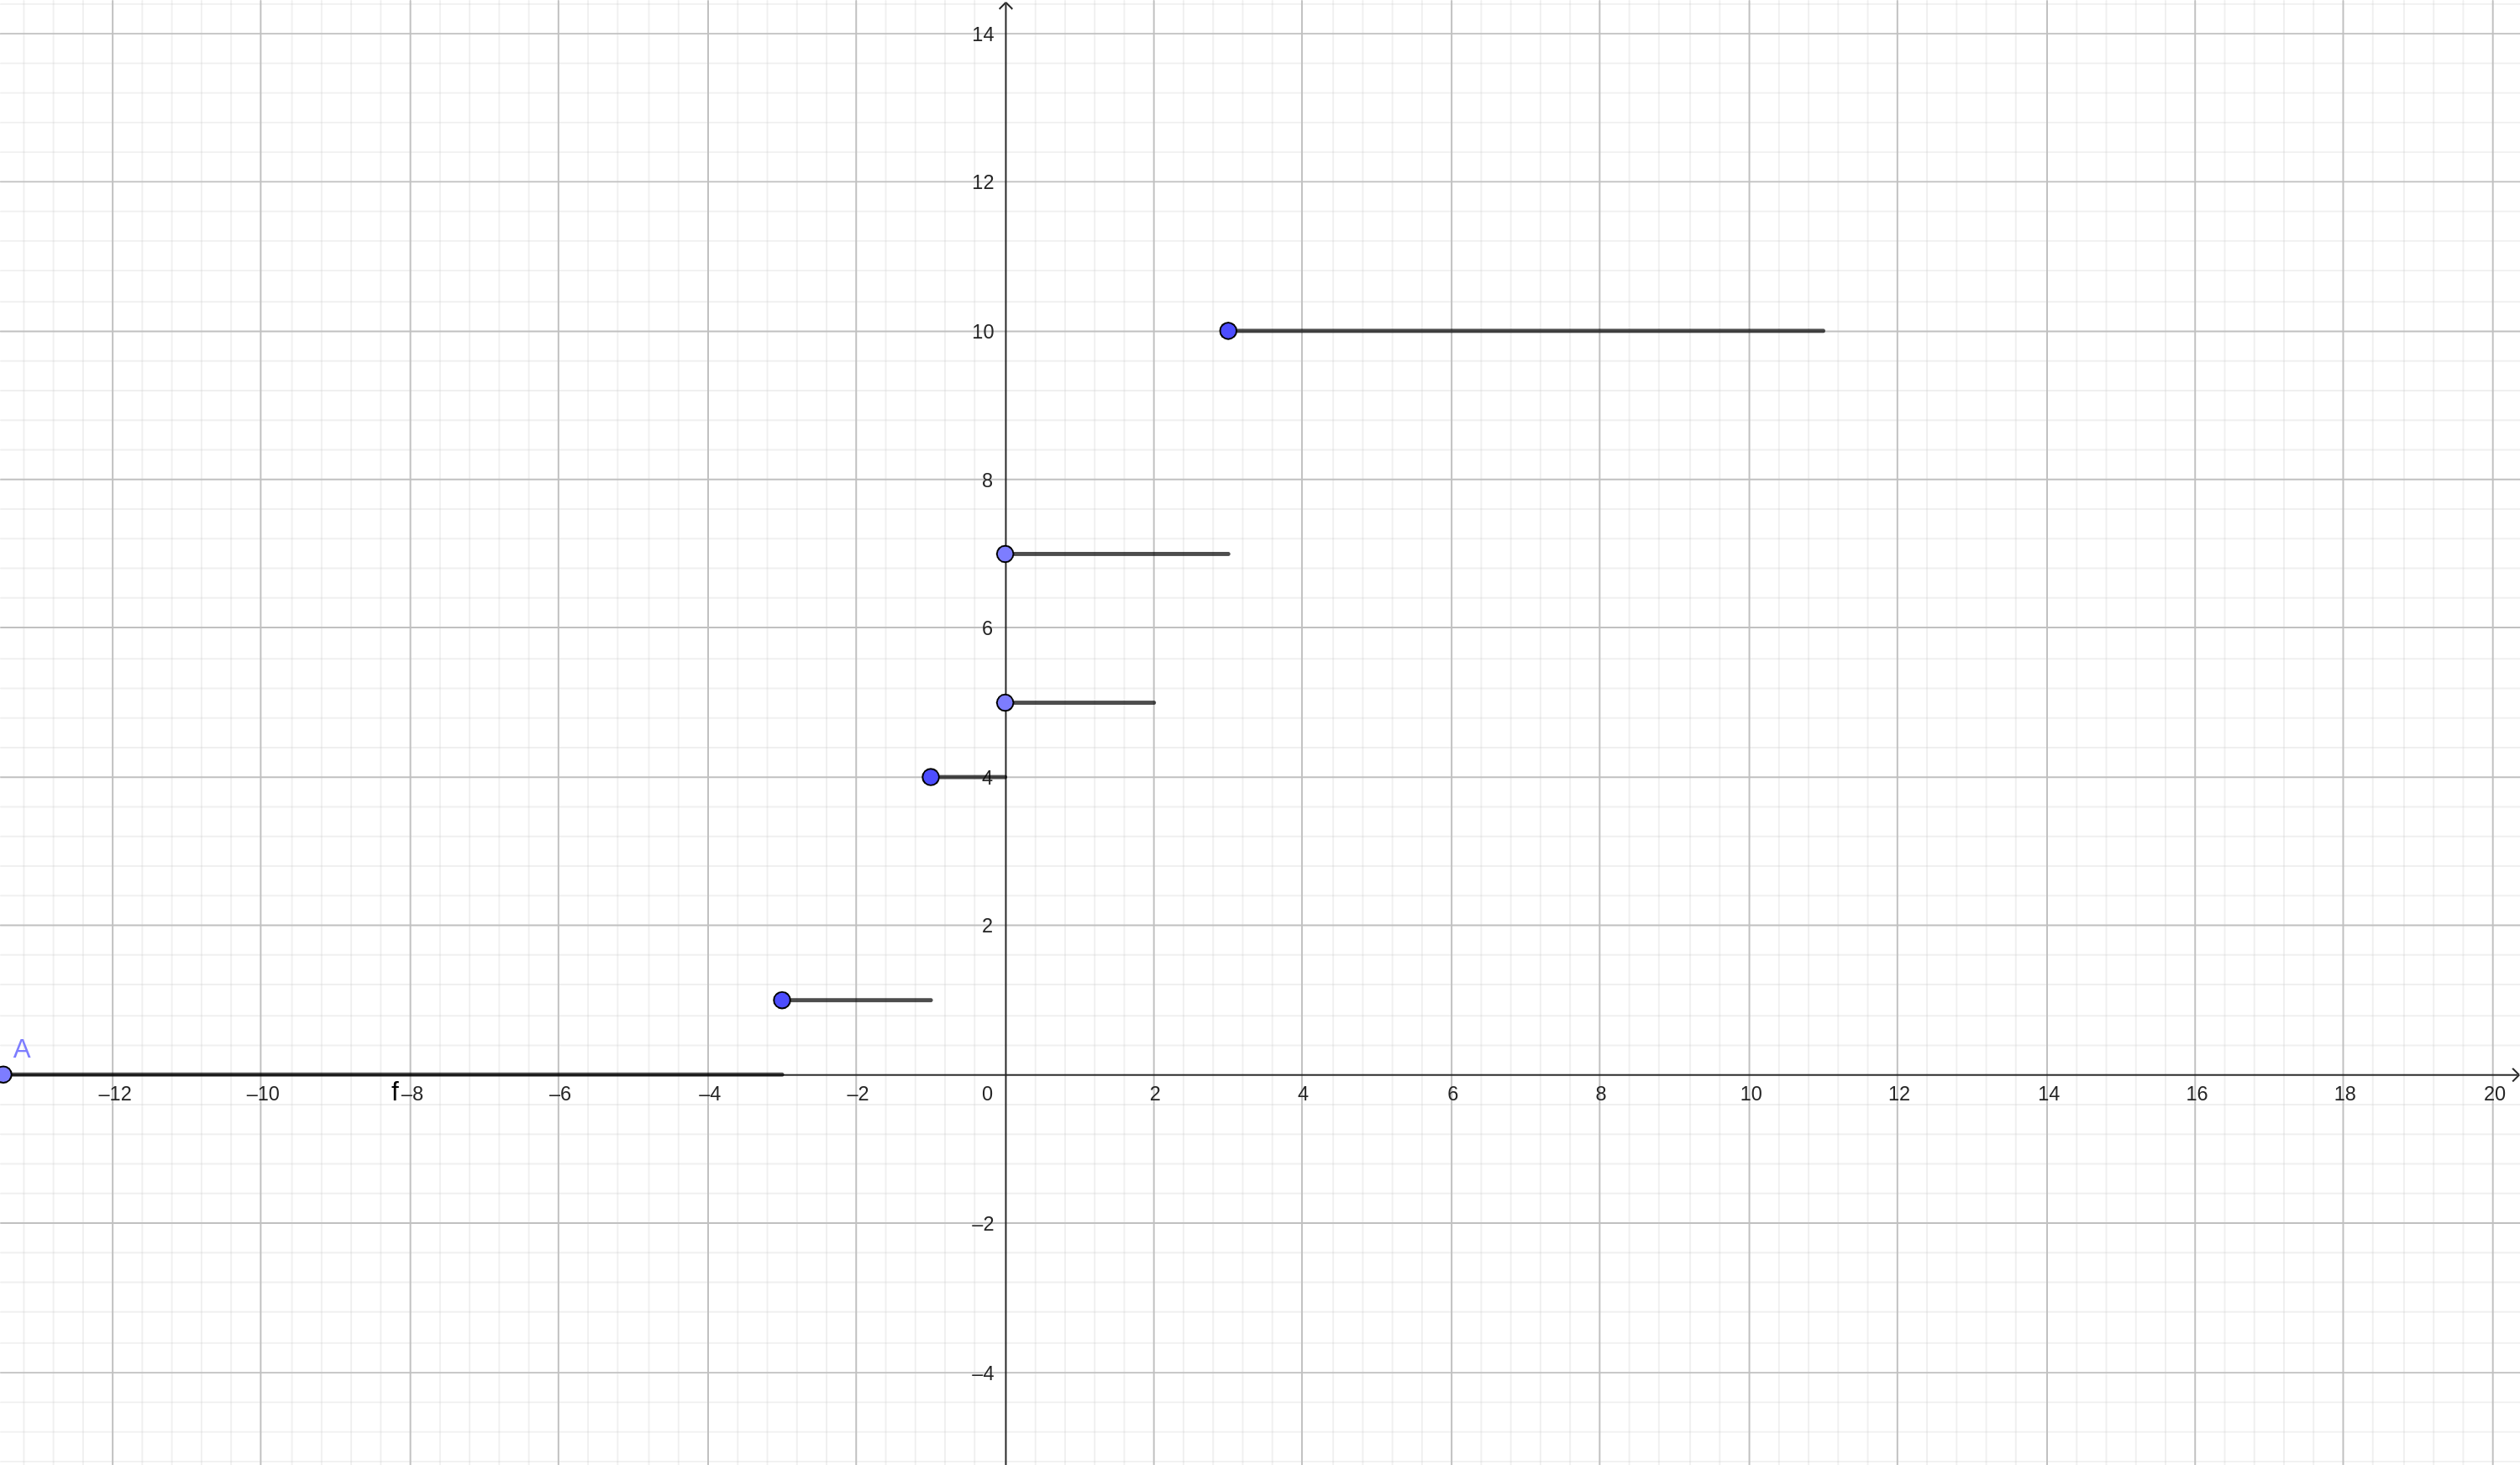
\includegraphics[width=0.8\textwidth]{repartition.png} % Remplacez par le chemin de votre image
    \label{fig:courbe_f}
\end{figure}


\subsection*{\underline{\textbf{\textcolor{red}{2. Loi de Binomiale}}}}

\subsection*{\underline{\textbf{\textcolor{red}{a. Loi de Bernouilli}}}}

Une variable aléatoire qui présente que 2 résultats possibles : succès (\(S\)) et échec (\(\overline{S}\)). 
Soit \(X\) la variable aléatoire qui prend \(1\) si (\(S\)) se réalise et \(0\) si (\(\overline{S}\)) se réalise.
On note par \(p = P(X = 1)\) et \(q = P(X = 0)\), on dit que \(X\) suit une loi de Bernoulli de paramètre \(p\).
On note \(X \sim B(p)\).

\textbf{Loi de probabilité de \( X \):}

\[
\begin{array}{|c|c|c|}
\hline
X_i & 0 & 1 \\
\hline
P_i & p & q \\
\hline
\end{array}
\]

\[
p + q = 1 \Rightarrow q = 1 - p
\]

\[
E(X) = p
\]

\[
V(X) = p - p^2 = p q
\]

\underline{\textbf{\textcolor{red}{Remarque}}}

Dans toute épreuve aléatoire, il est possible de définir une variable aléatoire qui suit une loi de Bernoulli. Il suffit de prendre un événement et son événement contraire.

\subsection*{\underline{\textbf{\textcolor{red}{b.Schéma de Bernoulli}}}}

Soit une épreuve aléatoire qui présente 2 issues possibles \( S \) et \( \overline{S} \), \( n \in \mathbb{N} \). Si la répétition successive et indépendante \( n \) fois de la même épreuve aléatoire est appelée schéma de Bernoulli.

\begin{tikzpicture}[level distance=5cm,
  level 1/.style={sibling distance=7cm}, % Ecarte les branches des 1ere ramifications
  level 2/.style={sibling distance=4cm}, % Ecarte les branches des 2eme ramifications
  level 3/.style={sibling distance=2cm}, % Ecarte les branches des 3eme ramifications
  every node/.style={text width=2cm, align=center}] % Permet de spécifier une largeur pour chaque nœud
  \node {}
    child {node {$\overline{S}$}
      child {node {$\overline{S}$}
        child {node {$\overline{S}$}}   % 1ère branche de $\overline{P}$
        child {node {$S$}}   % 2ème branche de $\overline{P}$
      }
      child {node {$S$}
        child {node {$\overline{S}$}}   % 1ère branche de $P$
        child {node {$S$}}   % 2ème branche de $P$
      }
    } % 1ère branche      
    child {node {$s$}  
      child {node {$\overline{s}$}
        child {node {$\overline{S}$}}   % 1ère branche de $\overline{P}$
        child {node {$S$}}   % 2ème branche de $\overline{P}$
      }
      child {node {$S$}
        child {node {$\overline{S}$}}   % 1ère branche de $P$
        child {node {$S$}}   % 2ème branche de $P$
      }
    };

  % Probabilités associées aux branches
  \node at (-3,-1.5) [right] {$q$};
  \node at (1,-1.5) [right] {$p$};

  \node at (-6,-7) [right] {$q$};
  \node at (-3,-7) [right] {$p$};

  \node at (4,-7) [right] {$p$};
  \node at (1,-7) [right] {$q$};

   \node at (3.5,-13) [right] {$q$};
  \node at (1.5,-13) [right] {$p$};
    \node at (5.5,-13) [right] {$p$};
  \node at (-0.5,-13) [right] {$q$};
  \node at (-1.5,-13) [right] {$p$};
  \node at (-4,-13) [right] {$q$};
    \node at (-5.5,-13) [right] {$p$};
  \node at (-8,-13) [right] {$q$};
\end{tikzpicture}

La variable aléatoire \( X \) qui prend le nombre de fois où l'événement succès s'est réalisé durant ces \( n \) répétitions suit une loi binomiale de paramètres \( n \) et \( p \), on note :\( X \sim B(n,p) \)

\(X(\Omega)=\{0,1,2,...,n\} \forall k \in X(\Omega)\)

\( P(X = k) = C_n^k p^k q^{n-k} \)

\[
\begin{array}{|c|c|c|c|c|c|}
\hline
X_i & 0 & 1 & 2 & \dots & n \\
\hline
P(X_i) & q^n & C_n^1 p^1 q^{n-1} & C_n^2 p^2 q^{n-2} & \dots & p^n \\
\hline
\end{array}
\]
\[
E(X) = n p
\]
\[
E(X) = n pq
\]

\underline{\textbf{\textcolor{red}{Exemple BAC 2004}}}

\end{document}